\documentclass{ieeeaccess}
\usepackage{cite}
\usepackage{amsmath,amssymb,amsfonts}
\usepackage{algorithm}
\usepackage{algpseudocode}
\usepackage{graphicx}
\usepackage{booktabs}
\usepackage{multirow}
\usepackage{textcomp}
\usepackage{url}
\usepackage{bm}
\makeatletter
\AtBeginDocument{\DeclareMathVersion{bold}
\SetSymbolFont{operators}{bold}{T1}{times}{b}{n}
\SetSymbolFont{NewLetters}{bold}{T1}{times}{b}{it}
\SetMathAlphabet{\mathrm}{bold}{T1}{times}{b}{n}
\SetMathAlphabet{\mathit}{bold}{T1}{times}{b}{it}
\SetMathAlphabet{\mathbf}{bold}{T1}{times}{b}{n}
\SetMathAlphabet{\mathtt}{bold}{OT1}{pcr}{b}{n}
\SetSymbolFont{symbols}{bold}{OMS}{cmsy}{b}{n}
\renewcommand\boldmath{\@nomath\boldmath\mathversion{bold}}}
\makeatother
\emergencystretch=2em

\begin{document}
\history{Date of publication xxxx 00, 0000, date of current version xxxx 00, 0000.}
\doi{10.1109/ACCESS.2024.0429000}

\title{Beyond Proximity: How Much of a 3D Scene Should a Language Model Read?
A Controlled Study of Hierarchical Context Reduction}
\author{\uppercase{Andrey Kuznetsov}\authorrefmark{1},
\uppercase{Mahmoud Mousatat}\authorrefmark{1},
\uppercase{Ahmad Taha}\authorrefmark{1},
\uppercase{Aleksandr Medvedev}\authorrefmark{1},
\uppercase{Leo Vesin}\authorrefmark{1},
\uppercase{Telman Nuruzov}\authorrefmark{1}, AND
\uppercase{Nikita Shankin}\authorrefmark{1}}
\address[1]{Independent researchers, Beyond Proximity project
(e-mail: medvedguk@gmail.com)}
\markboth
{Kuznetsov \headeretal: How Much of a 3D Scene Should a Language Model Read?}
{Kuznetsov \headeretal: How Much of a 3D Scene Should a Language Model Read?}
\corresp{Corresponding author: Aleksandr Medvedev
(e-mail: medvedguk@gmail.com).}

\begin{abstract}
Language interfaces to digital twins and robot maps increasingly hand the final
decision to a large language model (LLM) that reads serialized scene records.
We ask how much of a 3D scene such a model must read, and whether a spatial
hierarchy selects that evidence better than a flat cheap-first cascade. We
formalize a recall-controlled traversal, in which a cached proxy ranks branches,
an adaptive probability-mass gate keeps them, and a global safety shortlist
protects the proxy's best records, and evaluate it under same-scorer,
matched-budget controls on 125 labeled queries over five rendered scenes, on
155,535 ReferIt3D expressions from 1,436 ScanNet scenes, and on ScanNet and
Replica object maps. Four findings emerge. First, a cheap BGE proxy in front of
Qwen2.5-7B halves the model's input (2,236 to 1,090 tokens) and latency (5.7 to
2.9\,s) at a hit@3 cost of 0.027 (95\% CI [$-0.067$, 0]), and giving the model three retained records instead of all of them raises its
answer accuracy from 0.613 to 0.733 (+0.120, 95\% CI [0.013, 0.227]). Second, at a matched candidate budget, hierarchical selection is
not better than flat top-$N$ selection, and when proxy and scorer coincide it
places the target at the same rank as flat top-$k$ on every held-out query. Third, the safety
shortlist makes retrieval insensitive to the hierarchy: manual zones and
pose-based and raw RGB-D hierarchies are statistically indistinguishable, whereas
a fixed two-branch gate loses up to 0.096 hit@3. Fourth, at 155,535 records a
scene hierarchy without localization at best ties flat search, although 96.9\%
of flat misses there come from other scenes. We release all traces, and we document and correct an orientation error in a
Replica ground-truth box import that had understated predicted-map accuracy.
\end{abstract}

\begin{keywords}
3D scene graphs, hierarchical retrieval, context reduction, retrieval cascades,
large language models, open-vocabulary grounding, RGB-D scene understanding,
approximate nearest-neighbor search.
\end{keywords}

\titlepgskip=-15pt
\maketitle

% =========================================================================
\section{Introduction}
% =========================================================================
\PARstart{A}{sking} a building, a museum, or a robot map a question in natural
language---``where can I sit near reception?'', ``which exit is closest to the
stage?''---is becoming a routine interface to digital twins and mobile robots.
Current systems answer such queries in two stages. A perception stage turns
posed RGB-D captures into records: object instances with boxes and
captions~\cite{gu2023conceptgraphs,conceptfusion2023}, hierarchical
floor--room--object graphs~\cite{hovsg2024,hydra2022}, or language-embedded
fields~\cite{kerr2023lerf,langsplat2024}. A reasoning stage then serializes these
records into the prompt of an LLM or a vision--language model, which selects the
answer~\cite{bbq2024,rana2023sayplan}.

The reasoning stage is where cost and failure concentrate. Its price, latency,
and memory grow with the number of serialized records, and its accuracy can drop
when relevant evidence is buried in a long context~\cite{liu2024lostmiddle}. A
single room already yields tens of records; a building yields thousands. It is
therefore natural to prune the scene before the model reads it, and spatial
structure is an intuitive way to do so: ``near reception'' already rules out
most of a building. Scene-graph systems follow this intuition. SayPlan lets an
LLM collapse and expand a hierarchical graph~\cite{rana2023sayplan}, HOV-SG
matches queries hierarchically~\cite{hovsg2024}, and BBQ shortlists objects
before deductive reasoning~\cite{bbq2024}.

What is missing is a controlled answer to two questions. \emph{How much of a
scene does the reasoner need?} And \emph{does a spatial hierarchy select that
evidence better than a flat cascade}---a cheap retriever that simply passes its
top $N$ records to the expensive model, the standard design in text
search~\cite{colbert2020,plaid2022}? Published systems change the hierarchy, the
scorer, and the budget at once, so their gains cannot be attributed to the
hierarchy. They also rarely report how many records reach the reasoner, how many
tokens it reads, or how much proxy computation remains.

This paper answers both questions under explicit controls. We formalize a
recall-controlled traversal (Algorithm~\ref{alg:query}) as a strong
representative of hierarchical pruning: branches are ranked by a cached proxy,
kept by an adaptive probability-mass gate, and backed by a global safety
shortlist that guarantees the proxy's best records reach the reasoner. We derive
a cost model that states when such a cascade saves computation. We then compare
the traversal, always with the same leaf scorer and the same budget, against
exhaustive scoring, flat top-$k$, flat top-$N$ cascades, weaker hierarchical
gates, and HNSW~\cite{hnsw2020}, and we vary the hierarchy itself from
human-authored zones to pose-only, pose+semantic, and raw RGB-D constructions.

\paragraph{Contributions}
\begin{itemize}
\item A controlled evaluation protocol for context reduction over 3D scene
records, in which the leaf scorer, the retained budget, and the query set are
fixed and only candidate selection varies, with exact token accounting and
paired bootstrap intervals.
\item Evidence that the reasoner should read less: with Qwen2.5-7B, a BGE
cascade halves input tokens and latency at a hit@3 cost whose 95\% interval
ends at 0.067, and three retained records yield higher answer accuracy than the
full scene.
\item Evidence that, at a matched budget, a spatial hierarchy does not select
better evidence than a flat cascade, and that its safety shortlist makes
retrieval quality insensitive to how the hierarchy is built.
\item A 155,535-record scale study showing that scope, not similarity, limits
flat referential retrieval, and that a language-only scene gate does not recover
the scope gain.
\item A release of all per-query traces, including a corrected Replica
ground-truth box import and the diagnostics that located the error.
\end{itemize}

Section~\ref{sec:related} reviews related work, Section~\ref{sec:method} defines
the traversal and the cost model, Section~\ref{sec:setup} describes the data and
protocol, Section~\ref{sec:results} reports results, and
Section~\ref{sec:discussion} discusses what they imply for spatial language
interfaces.

% =========================================================================
\section{Related Work}
\label{sec:related}
% =========================================================================

\subsection{Language-aligned 3D scene representations}
A first family of methods attaches language features directly to a dense scene
representation. LERF~\cite{kerr2023lerf} distills CLIP~\cite{radford2021clip}
features into a neural radiance field, and LangSplat~\cite{langsplat2024},
Semantic Gaussians~\cite{semanticgaussians2024}, and LEGS~\cite{legs2024} do the
same for 3D Gaussian splatting~\cite{kerbl20233dgs}.
OpenScene~\cite{openscene2023} and ConceptFusion~\cite{conceptfusion2023} fuse
open-vocabulary features into point clouds. These representations answer a query
by dense feature matching over the whole scene and do not produce discrete
records that an LLM reads. Our study is complementary: it assumes that a
perception stage has produced discrete records and asks how many of them the
reasoning stage needs.

\subsection{3D scene graphs and hierarchical reasoning}
Scene graphs make that discretization explicit. 3DSSG~\cite{wald20203dssg}
learns object--relation graphs from indoor reconstructions;
Hydra~\cite{hydra2022} builds real-time layered graphs from objects to places,
rooms, and buildings; and Clio~\cite{maggio2024clio} adapts graph granularity to
the task. ConceptGraphs~\cite{gu2023conceptgraphs} builds open-vocabulary object
graphs from RGB-D and passes captioned objects to an LLM planner.
BBQ~\cite{bbq2024}, the closest object-grounding reference to our work, adds
deductive LLM reasoning over a 3D object graph and reports Acc@$\tau$ on Replica
and ScanNet. HOV-SG~\cite{hovsg2024} and Search3D~\cite{takmaz2025search3d}
organize open-vocabulary content into floor--room--object or part--object
hierarchies for navigation and segmentation. SayPlan~\cite{rana2023sayplan} is
closest in spirit: an LLM collapses and expands a hierarchical 3D scene graph so
that large environments fit in context. It reports the tokens saved by
collapsing, but not the quality lost by pruning for a fixed scorer. None of these
systems isolates the contribution of the hierarchy from that of the scorer and
the budget. Table~\ref{tab:qualitative} summarizes the differences; numerical
comparisons are restricted to same-input methods in Section~\ref{sec:objects}.

\begin{table*}[!t]
\centering
\caption{Qualitative comparison with representative systems. ``LLM calls''
counts calls per query at inference time. ``Controlled'' indicates whether the
paper compares pruning against flat selection with the same scorer and budget,
and reports retained records and tokens.}
\label{tab:qualitative}
\footnotesize
\setlength{\tabcolsep}{4pt}
\begin{tabular}{p{0.15\textwidth}p{0.13\textwidth}p{0.15\textwidth}p{0.19\textwidth}ccc}
\toprule
Method & Input & Scene structure & Query-time selection & Open vocab. &
LLM calls & Controlled \\
\midrule
ConceptGraphs~\cite{gu2023conceptgraphs} & posed RGB-D & object graph (flat) &
full graph to LLM & yes & 1 & no \\
BBQ~\cite{bbq2024} & posed RGB-D & object graph (flat) & object shortlist +
deductive LLM & yes & $\geq$2 & no \\
HOV-SG~\cite{hovsg2024} & posed RGB-D & floor--room--object & hierarchical CLIP
matching & yes & 1 (parsing) & no \\
SayPlan~\cite{rana2023sayplan} & given 3D scene graph & floor--room--asset & LLM
expand/collapse & yes & many (iterative) & partial \\
RAPTOR~\cite{raptor2024} & text chunks & summary tree & embedding over tree &
yes & 0 (retrieval) & no \\
\textbf{This study} & posed RGB-D, object maps, expressions & zone or scene
branches (manual or automatic) & proxy gate + safety shortlist vs.\ flat
cascades & via scorer & 0--1 & yes \\
\bottomrule
\end{tabular}
\end{table*}

\subsection{Language grounding benchmarks in 3D}
ScanRefer~\cite{scanrefer2020} and ReferIt3D~\cite{referit3d2020} established
referring-expression grounding in ScanNet reconstructions~\cite{scannet2017},
and Multi3DRefer~\cite{multi3drefer2023} generalized it to zero or multiple
targets. ScanQA and SQA3D~\cite{scanqa2021,sqa3d2022} extended the same scenes to
question answering, while 3DRefTransformer and ScanEnts3D
\cite{reftransformer2022,scanents3d2024} learn phrase--object correspondences.
OpenLex3D~\cite{openlex3d2025} argues for tiered evaluation of open-vocabulary
representations. These benchmarks measure whether the right object is found,
not how much of the scene had to be examined. We reuse the ReferIt3D expressions
and the BBQ scene subset and add that cost axis. For object maps predicted from
RGB-D, OpenMask3D, Open3DIS, and Mask3D~\cite{openmask3d2023,open3dis2024,
mask3d2023} are alternative instance predictors to the ConceptGraphs maps used
here.

\subsection{Context reduction and retrieval cascades}
In text retrieval-augmented generation, prompt compression and context pruning
\cite{promptcompression2024,longllmlingua2023,recomp2023,provence2025,
attentionrag2025} reduce the tokens given to a generator, and RAPTOR and GraphRAG
\cite{raptor2024,edge2024graphrag} organize corpora into trees or communities.
Cascades of a cheap retriever and an expensive reranker are standard in text
search, and ColBERT and PLAID~\cite{colbert2020,plaid2022} make the
efficiency--quality trade-off of late interaction explicit. HNSW and FAISS
\cite{hnsw2020,faiss2019} accelerate the first stage itself. Our traversal is a
cascade whose first stage is shaped by 3D containment; the central question of
this paper is whether that shaping adds anything over a flat first stage.
Tool-using LLMs~\cite{react2023,toolformer2023} motivate our system interface, in
which the traversal is exposed as a tool, but no reported number depends on a
particular client.

% =========================================================================
\section{Method}
\label{sec:method}
% =========================================================================

\subsection{Problem formulation and notation}
A scene is represented by a rooted hierarchy $H=(V,E)$. Its \emph{leaves}
$\mathcal{L}\subset V$, $|\mathcal{L}|=N$, are \emph{records}: posed RGB-D
\emph{views} (internal benchmark), \emph{object instances} (public object maps),
or \emph{expressions} (scale study). Each record carries searchable text and,
where available, 3D boxes, spatial relations, and links to supporting
observations. Internal nodes are \emph{branches} (zones, regions, or scenes);
$C_b\subseteq\mathcal{L}$ denotes the records under branch $b$, and $M$ the
number of top-level branches. Branches may overlap in the manual reference and
are disjoint in automatic hierarchies.

A query $q$ is answered by a \emph{leaf scorer} $r(q,\ell)$ that ranks records.
The \emph{exhaustive} baseline scores all $N$ records with $r$. A
\emph{candidate-selection} method passes a subset $C(q)\subseteq\mathcal{L}$ to
$r$ and keeps the top $k$ records, the \emph{budget}. Records in $C(q)$ are
\emph{retained}, and the text serialized from them is the \emph{context}.
Selection uses a cheap \emph{proxy} score $s(q,\ell)$ that is precomputed or
cached per record. The two flat baselines are \emph{flat top-$k$}, which keeps
the top $k$ records under $r$, and the \emph{flat cascade} top-$N_q$, which
passes the top $N_q$ records under $s$ to $r$, with $N_q$ matched per query to
$|C(q)|$. Table~\ref{tab:notation} fixes this vocabulary; each term is used for
one concept only.

\begin{table}[!t]
\centering
\caption{Notation and terminology.}
\label{tab:notation}
\footnotesize
\begin{tabular}{p{0.24\columnwidth}p{0.66\columnwidth}}
\toprule
Symbol / term & Meaning \\
\midrule
record, leaf $\ell$ & a view, object, or expression; the unit that is scored \\
branch $b$, $C_b$ & a zone, region, or scene; the records it contains \\
$N$, $M$ & number of records; number of top-level branches \\
$s(q,\ell)$ & cheap proxy score (cached) \\
$r(q,\ell)$ & leaf scorer (lexical, BGE, CLIP, or LLM) \\
$g_b(q)$, $p_b(q)$ & branch score; branch probability \\
$\tau$, $T$, $B$ & probability-mass target, temperature, branch cap \\
$m$ & size of the global safety shortlist \\
$C(q)$, $N_q$ & retained candidate set; its size \\
$k$ & budget: records returned after rescoring \\
context & serialized text read by the scorer or reasoner \\
\bottomrule
\end{tabular}
\end{table}

\subsection{Recall-controlled traversal}
\label{sec:traversal}
\paragraph{Branch scoring}
We consider two branch scores. The \emph{max-leaf} score ranks a branch by its
best record,
\begin{equation}
 g_b(q)=\max_{\ell\in C_b}s(q,\ell),
 \label{eq:maxleaf}
\end{equation}
which avoids the bias of concatenated branch text against large branches but
costs $O(N)$. The \emph{summary} score ranks a branch by the proxy similarity
between the query and a cached branch summary---the zone description for views,
or the normalized mean record embedding for scenes---which costs $O(M)$. Branch
scores are converted into probabilities with temperature $T$,
\begin{equation}
 p_b(q)=\frac{\exp(g_b(q)/T)}{\sum_{j}\exp(g_j(q)/T)}.
 \label{eq:softmax}
\end{equation}

\paragraph{Adaptive gate and safety shortlist}
Branches are kept in descending $p_b$ until their cumulative probability reaches
$\tau$ or $B$ branches are kept, so a query whose evidence is concentrated in one
zone keeps one branch and an ambiguous query keeps several. Because any gate can
drop the correct branch, the candidate set also contains the global top-$m$
records under the proxy, $\operatorname{Top}_m(s)$; with $m\geq1$ the proxy's
best record always reaches the scorer. The leaf scorer then ranks $C(q)$ and the
top $k$ records are returned (Algorithm~\ref{alg:query}). Every quantity the
algorithm computes is written to a per-query trace.

\begin{algorithm}[!t]
\caption{Recall-controlled query traversal}
\label{alg:query}
\small
\begin{algorithmic}[1]
\Require hierarchy $H$ with branches $\{C_b\}$; query $q$; proxy $s$; leaf
scorer $r$; parameters $\tau, T, B, m, k$
\Ensure ranked records $R_k$; trace
\State compute branch scores $g_b$ (max-leaf or summary)
\State $p_b\gets\operatorname{softmax}_b(g_b/T)$; sort branches by $p_b$
\State $S\gets\emptyset$;\quad $P\gets 0$
\For{each branch $b$ in that order}
 \State $S\gets S\cup\{b\}$;\quad $P\gets P+p_b$
 \If{$P\geq\tau$ \textbf{or} $|S|=B$} \textbf{break} \EndIf
\EndFor
\State $C\gets\bigcup_{b\in S}C_b\;\cup\;\operatorname{Top}_m(s)$
\State $R_k\gets$ top-$k$ of $C$ under $r(q,\cdot)$
\Comment{$|C|$ scorer calls}
\State write $p_b$, $S$, $C$, proxy count, context tokens, and $R_k$ to the trace
\State \Return $R_k$
\end{algorithmic}
\end{algorithm}

\paragraph{Parameter selection}
All traversal parameters are selected on a frozen 50-query development split
(Section~\ref{sec:setup}). For the lexical scorer, development tuning selected
max-leaf branch scores with $(\tau,T,B,m)=(0.7,0.25,5,1)$; for BGE it selected
summary branch scores with $(0.5,0.1,5,1)$. The budget $k$ is the smallest value
whose paired hit@3 difference to exhaustive scoring has a 95\% bootstrap lower
bound of at least $-0.05$ on the development split, that saves at least 25\% of
records, and that excludes at least 20\% of branches on average. For the lexical
scorer this criterion selects $k=3$. For BGE no budget meets it on the
development split, where the traversal misses one query that flat search finds
(lower bound $-0.06$); we use $k=3$ for BGE as well and report the consequence.
A confidence fallback to exhaustive scoring and soft boundary membership were
also evaluated on the development split and rejected (Section~\ref{sec:ablation}).

\subsection{Cost model}
\label{sec:complexity}
Let $c_p$ and $c_s$ be the costs of one proxy and one leaf-scorer evaluation.
Exhaustive scoring costs $Nc_s$. With max-leaf scores, Algorithm~\ref{alg:query}
costs $Nc_p+O(M)$ for the proxy and gate plus $N_qc_s$ for rescoring; with
summary scores and an approximate top-$m$ shortlist, the proxy term drops to
$O(M)$ plus the cost of the approximate search. The cascade reduces computation
only if
\begin{equation}
 Nc_p+N_qc_s<Nc_s
 \;\Longleftrightarrow\;
 \frac{N_q}{N}<1-\frac{c_p}{c_s}.
 \label{eq:breakeven}
\end{equation}
Two consequences shape the evaluation. First, when the proxy and the leaf scorer
are the same function ($s\equiv r$), rescoring adds no information: the shortlist
already contains the global top-$m$ records, and the traversal can at best
reproduce flat top-$k$. We therefore report flat top-$k$ as the fair baseline in
that regime and treat the comparison as a correctness check. Second, the regime
in which Eq.~\eqref{eq:breakeven} holds by a wide margin is an LLM scorer, whose
per-record cost exceeds that of a cached embedding lookup by orders of magnitude.
There, any cascade saves computation, so the relevant baseline is the flat
cascade with the same $N_q$; the question is whether the hierarchy chooses
better records.

\subsection{Hierarchy construction}
\label{sec:construction}
We compare four hierarchies over the same 97 internal views. None of the
automatic constructors reads the manual zones, and each writes its hierarchy to
disk before the evaluator opens them; a source ledger records every file read.

\paragraph{Manual reference}
Twenty-six human-authored zones over the five scenes, which may overlap, together
with per-view semantic records (1,066 items in total) written by the authors.

\paragraph{Pose only and pose+semantic}
Views are connected when their camera translations $p_i$ are closer than an
adaptive threshold,
\begin{equation}
 t=\alpha\cdot\operatorname{median}_i\min_{j\neq i}\lVert p_i-p_j\rVert_2,
 \qquad \alpha=3.5,
 \label{eq:threshold}
\end{equation}
and connected components form branches. Normalizing by the median
nearest-neighbor spacing makes the threshold independent of capture scale and
density. The multiplier $\alpha$ was fixed before evaluation, and
Table~\ref{tab:constants} reports its effect. Pose-only reads only the camera
poses. Pose+semantic additionally merges components whose authored view records
share a complementary facing pair, or both a room type and a landmark; it
therefore reads the authored records, but not the zones. At $\alpha=3.5$,
pose-only yields a single branch in two of the three indoor scenes and
pose+semantic in all three, so both hierarchies are coarse.

\paragraph{Raw RGB-D}
The strictest constructor reads only RGB images, depth maps, and poses. For each
view it computes a frozen CLIP ViT-B/32 image embedding~\cite{radford2021clip}
$f_i\in\mathbb{R}^{512}$, the camera translation $p_i\in\mathbb{R}^3$, and a
depth descriptor $d_i\in\mathbb{R}^6$ (valid-depth ratio and five depth
quantiles). The concatenated features $[f_i;p_i;d_i]$ are standardized per
dimension and clustered with $k$-means from a deterministic farthest-point
initialization; the number of clusters $K\in\{2,\ldots,\lfloor n/3\rfloor\}$
maximizes the silhouette score, where $n$ is the number of views in the scene.
Because every dimension is standardized, pose and depth contribute 9 of 521
equally weighted dimensions, and appearance dominates the grouping. Per-block weights applied before this standardization would cancel, so none
are used; the constructor also enforces no minimum cluster size, and the
resulting hierarchy contains nine single-view clusters (Table~\ref{tab:constants}
reports both choices). Each cluster is named by the nearest of 20
place categories in CLIP text space (Appendix~\ref{app:vocab}). Names only label
branches in traces and play no role in retrieval; both clusters of the drone
flight receive the indoor label ``stage''. Algorithm~\ref{alg:construction}
summarizes the protocol.

\begin{algorithm}[!t]
\caption{Raw RGB-D hierarchy construction}
\label{alg:construction}
\small
\begin{algorithmic}[1]
\Require RGB frames $\{I_i\}$, depth maps $\{D_i\}$, poses $\{P_i\}$ of one scene
\Ensure disjoint branches with names; source ledger
\State verify that frames, depths, and poses are aligned
\State compute $f_i$ (CLIP), $p_i$ (translation), $d_i$ (depth descriptor)
\State $z_i\gets$ per-dimension standardization of $[f_i;p_i;d_i]$
\For{$K=2,\ldots,\lfloor n/3\rfloor$}
 \State cluster $\{z_i\}$ into $K$ groups; record the silhouette score
\EndFor
\State keep the $K$ with the highest silhouette score
\State name each cluster by the nearest place category in CLIP text space
\State serialize hierarchy and ledger; only then open evaluation labels
\end{algorithmic}
\end{algorithm}

\subsection{Leaf scorers}
\label{sec:scorers}
\paragraph{Lexical and dense scorers}
The lexical scorer normalizes case, stop words, aliases, and plurals and ranks by
token overlap plus overlap divided by query length, breaking ties by record ID.
The dense scorer is the cosine similarity of BGE-small-en-v1.5
embeddings~\cite{cpack2024}. For both, the record proxy $s$ is the same function
as the leaf scorer $r$, which places them in the $s\equiv r$ regime of
Section~\ref{sec:complexity}.

\paragraph{Instruction-model scorer}
The expensive scorer is Qwen2.5-7B-Instruct~\cite{qwen25report}; an additional
Qwen2.5-1.5B-Instruct run on a CPU is reported for reference. For query
$q$ and record $c$ the model receives
\begin{quote}\small\ttfamily\raggedright
Judge scene-query relevance using semantic meaning and affordances.
Answer exactly Yes or No.\par
Query: <q>. Candidate: <c>. Relevant? Answer exactly Yes or No.
\end{quote}
and records are ranked by the log-odds of the next token \texttt{Yes} versus
\texttt{No}. All prompts of one query are scored in a single batched forward
pass. In the cascades, the BGE proxy selects $C(q)$ and Qwen rescores only
$C(q)$. As an ablation we also evaluate an LLM-only gate that first asks the same
question about each top-level branch description, keeps the two branches with the
highest score, and then scores their records; it needs two model invocations per
query.

\paragraph{Image--text scorer}
For hierarchy comparisons that must not depend on authored text, CLIP ViT-B/32
text embeddings score view images directly.

\paragraph{Object grounding}
On object maps, a rule-based parser produces a target phrase, an optional
relation (near, left/right, above/below, front/behind), and an optional anchor.
The base score combines exact-label match, lexical overlap, object type, and a
fixed affordance lexicon, capped at 1. A relation verified from stored links or
box centers adds $0.2$, and relation status breaks ties among equally scored
objects. In the queries studied here every relation-bearing top candidate already
reaches the cap, so relations act only as a tie-breaker, and sweeping the bonus
over $\{0.2,0.35,0.5\}$ or the fallback threshold below over $\{0.35,0.45,0.55\}$
leaves Acc@0.25 unchanged. If the best score is below $0.45$, the geometry is
invalid, or a required relation is unresolved, the candidate set is expanded to
all objects.

\subsection{System interface}
The traversal and the constructors are exposed as tools through a Model Context
Protocol (MCP) server, so that an interactive LLM client can build and query
hierarchies. We used this interface for qualitative demonstrations only; every
number in this paper is produced by the released scripts with the open models
listed in Section~\ref{sec:repro}.

% =========================================================================
\section{Experimental Setup}
\label{sec:setup}
% =========================================================================

\subsection{Internal benchmark}
The internal benchmark is built from five 3D Gaussian splatting
reconstructions~\cite{kerbl20233dgs}: a conference hall, a museum, a theater, an
outdoor street, and an aerial scene around an island (Fig.~\ref{fig:scenes}). The reconstructions are public scenes from the SuperSplat platform
(\url{https://superspl.at}); scene titles, authors, and links are listed in the
release. An operator placed 97 camera poses interactively in
a browser viewer, and an RGB image and a depth map were rendered from the
reconstruction at each pose, so depth is renderer-derived rather than measured by
a sensor, and rendering artifacts of the reconstructions are part of the input. The authors wrote 150 queries covering object
names, attributes, affordances, spatial relations, and multi-hop descriptions;
125 have a verified set of expected views and 25 are negatives whose target does
not occur in the scene. The 125 positives are split once, before any tuning, into
50 development and 75 test queries, stratified by scene and query type. The
queries, expected views, and negatives were written and checked within the
project and have not been relabeled by independent annotators.

\begin{figure*}[!tbp]
\centering
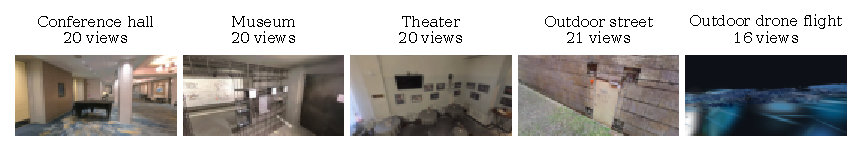
\includegraphics[width=0.98\textwidth]{figures/fig_scene_gallery.pdf}
\caption{The five scenes of the internal benchmark, rendered from 3D Gaussian
splatting reconstructions, with the number of posed RGB-D views per scene.}
\label{fig:scenes}
\end{figure*}

\subsection{Public benchmarks}
Following the BBQ scene subset~\cite{bbq2024}, we use eight Replica scenes
(room0--2, office0--4; 575 official boxes; 48 positive and 8 negative queries)
and eight ScanNet scenes (0011\_00, 0030\_00, 0046\_00, 0086\_00, 0222\_00,
0378\_00, 0389\_00, 0435\_00; 392 official boxes) with 48 Nr3D/Sr3D+
queries~\cite{referit3d2020} and an extended track that adds 8 positives and 8
negatives. The 48 ScanNet queries were used while the object scorer was
developed, so all ScanNet object-grounding results are in-sample. Object
grounding is evaluated on \emph{oracle maps}, which contain the official object
IDs and boxes and isolate retrieval, and on \emph{predicted maps}, produced by
ConceptGraphs~\cite{gu2023conceptgraphs} from 3--7 sampled RGB-D frames per
scene.

\paragraph{Replica ground-truth correction}
Replica stores each object box in its local frame together with a rotation. Our initial importer read the local box as a world-frame box and dropped the
rotation, whose per-scene median is between 12\textdegree{} and
76\textdegree{}. Rotating the boxes into the world frame raises the median best
IoU between the saved predicted boxes and the ground truth from 0.065 to 0.407
and reduces the median distance from a target to the nearest predicted box of the
same label from 1.56\,m to 0.36\,m. Feeding the ground-truth boxes through the
evaluation as predictions yields Acc@0.25 and Acc@0.5 of 1.000 on both datasets.
ScanNet boxes share the axis-aligned frame of the predictions, and no correction
was needed there. All Replica predicted-map numbers below use the corrected
boxes.

\subsection{Scale study}
We index all 155,535 Nr3D and Sr3D+ expressions from 1,436 ScanNet scenes
(16,650 objects) in nested pools of 1,000, 10,000, 50,000, 100,000, and 155,535
records. A query is an expression whose own record is removed from the pool; a
hit is another expression of the same scene and object. This is
expression-to-expression retrieval, a proxy for retrieving text-described object
records, not 3D box grounding. Each pool evaluates up to 500 queries (88 at the
1,000 pool, where few objects have two expressions), 2,088 query--pool pairs in
total. Hierarchy parameters are tuned on 2,000 further query--pool pairs that do
not overlap the evaluation queries.

\subsection{Metrics and statistics}
View retrieval uses hit@1, hit@3, and mean reciprocal rank (MRR) over positive
queries; for methods that return $k$ records, MRR is computed over the returned
list. Answer accuracy is the fraction of queries for which the model's chosen
record is an expected view. Object grounding uses exact-ID Recall@$k$ and
Acc@$\tau$, the fraction of positive queries whose top-ranked box has 3D IoU of at
least $\tau$ with the ground truth; negatives have no box, are excluded from these
denominators, and are evaluated by negative accuracy, the fraction for which the
system abstains. Structural agreement with the manual zones uses macro pairwise
F1 over co-clustered view pairs, reported beside a cluster-size-matched random
partition and the best disjoint projection of the overlapping manual zones.
Context tokens of view records are counted with the \texttt{cl100k\_base}
tokenizer for all non-LLM scorers and with the Qwen tokenizer for Qwen; object-map
tokens are character/4 estimates. Construction cost is reported separately from
query cost. Differences between methods are paired by query, with 95\% intervals
from 10,000 bootstrap resamples; single proportions use Wilson intervals.

% =========================================================================
\section{Results}
\label{sec:results}
% =========================================================================

\subsection{An LLM reasoner should read less}
\label{sec:llm}
Table~\ref{tab:llm} and Fig.~\ref{fig:llm} evaluate the regime in which
Eq.~\eqref{eq:breakeven} predicts a benefit: Qwen2.5-7B scores the records, and a
BGE proxy decides which records it reads. Scoring all 19.4 records per query costs
2,236 input tokens and 5.7\,s per query at hit@1/hit@3 of 0.627/0.973 on the 75
held-out positives. Algorithm~\ref{alg:query} retains 9.48 records, halves the
input to 1,090 tokens and the latency to 2.9\,s, and obtains 0.653/0.947. The
paired hit@3 difference is $-0.027$ (95\% CI $[-0.067,0.000]$) and the hit@1
difference $+0.027$ ($[-0.040,0.107]$). Truncating the proxy ranking to three
records before the LLM reads them cuts the input to 338 tokens and the latency to
0.86\,s at 0.640/0.960. The LLM-only two-branch gate is the worst selector: it
reads more (1,767 tokens in two calls) and loses more (hit@3 0.880), because the
target falls outside its two branches for 9.3\% of queries. The Qwen2.5-1.5B CPU run shows the same pattern for that gate (hit@3 0.867
versus 0.907 on the same test queries). On all 125 positives, including the
development queries, the hit@3 cost of Algorithm~\ref{alg:query} relative to
exhaustive scoring is 0.032 (95\% CI $[-0.064,-0.008]$), so a small recall loss
is real.

\begin{table*}[!t]
\centering
\caption{LLM leaf scorer (Qwen2.5-7B-Instruct, bfloat16, Apple M4 Pro GPU) on the
75 held-out positives. ``Retained'' is the number of records the LLM scores;
tokens are native Qwen input tokens per query; latency is the median wall time per
query including the proxy. Rows (b) and (c) retain the same number of records per
query, as do rows (d) and (e). Paired differences (95\% CI): (c)$-$(a) hit@3
$-0.027$ $[-0.067,0.000]$; (c)$-$(b) hit@3 $-0.013$ $[-0.040,0.000]$ and hit@1
$0.000$ $[-0.067,0.067]$; (e)$-$(d) zero for every metric.}
\label{tab:llm}
\footnotesize
\begin{tabular}{llccccccc}
\toprule
& Candidate selection before the LLM & hit@1 & hit@3 & MRR & Target in $C$ &
Retained & Tokens & Latency (s) \\
\midrule
(a) & none (all records) & 0.627 & 0.973 & 0.796 & 1.000 & 19.40 & 2,236 & 5.68 \\
(b) & flat BGE top-$N_q$ & 0.653 & 0.960 & 0.800 & 0.987 & 9.48 & 1,090 & 2.89 \\
(c) & Algorithm~\ref{alg:query}, summary gate & 0.653 & 0.947 & 0.793 & 0.973 &
9.48 & 1,090 & 2.87 \\
(c$'$) & Algorithm~\ref{alg:query}, max-leaf gate & 0.693 & 0.960 & 0.819 & 0.987
& 13.47 & 1,550 & 3.90 \\
(d) & flat BGE top-3 & 0.640 & 0.960 & 0.784 & 0.960 & 3.00 & 345 & 0.81 \\
(e) & Algorithm~\ref{alg:query}, $k=3$ & 0.640 & 0.960 & 0.784 & 0.960 & 2.95 &
338 & 0.86 \\
(f) & LLM-only two-branch gate & 0.653 & 0.880 & 0.757 & 0.907 & 11.15 & 1,767 &
4.34 \\
\bottomrule
\end{tabular}
\end{table*}

\begin{figure*}[!tbp]
\centering
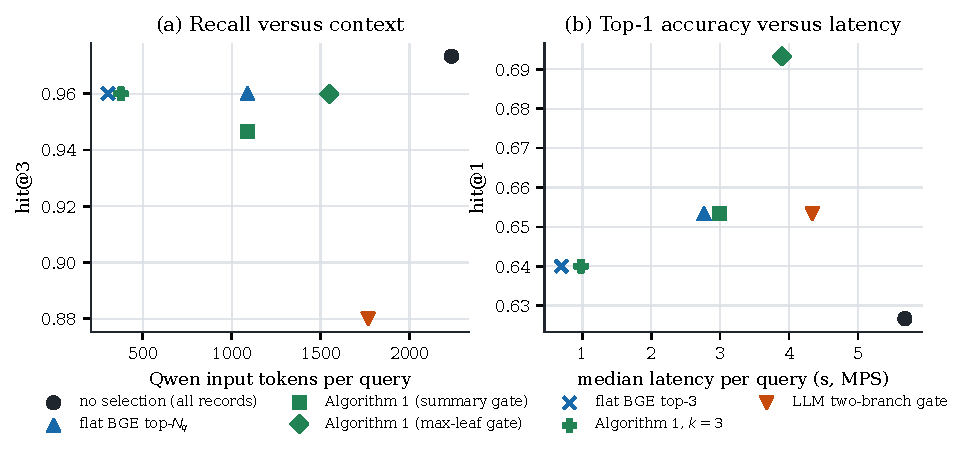
\includegraphics[width=0.96\textwidth]{figures/fig_llm_cascade.pdf}
\caption{Candidate selection in front of Qwen2.5-7B on the 75 held-out positives.
(a) hit@3 against the number of input tokens the LLM reads; (b) hit@1 against
median latency per query. Coinciding points are offset horizontally for
visibility (see Table~\ref{tab:llm} for exact values).}
\label{fig:llm}
\end{figure*}

A shorter context also helps when the model must commit to one answer. Given the
query and a numbered list of records, Qwen2.5-7B outputs one record identifier by
greedy decoding (Table~\ref{tab:answer}). With decoding constrained to identifiers
that occur in the list, it selects an expected record for 0.613 of the held-out
queries when it reads all 19.4 records and for 0.733 when it reads the three
records retained by Algorithm~\ref{alg:query} ($+0.120$, 95\% CI
$[0.013,0.227]$); flat BGE top-3 gives the same 0.733. With unconstrained
decoding the gap is similar (0.587 versus 0.720), and the full list additionally
produces invalid identifiers for 13\% of queries. The constrained decoder was
added after the unconstrained run had been inspected; both are reported. The
short-context conditions forgo only the 4\% of queries whose target is outside
the three retained records.

\begin{table}[!t]
\centering
\caption{Answer selection by Qwen2.5-7B on the 75 held-out positives: the model
reads the query and a numbered list of records and outputs one record ID, with
decoding constrained to listed IDs or unconstrained (free).}
\label{tab:answer}
\footnotesize
\setlength{\tabcolsep}{3pt}
\begin{tabular}{lcccc}
\toprule
& \multicolumn{2}{c}{Accuracy} & & \\
\cmidrule{2-3}
Context & constr. & free (valid) & Records & Tokens \\
\midrule
all records & 0.613 & 0.587 (0.867) & 19.40 & 1,343 \\
flat BGE top-3 & 0.733 & 0.707 (0.960) & 3.00 & 266 \\
Alg.~\ref{alg:query}, $k=3$ & 0.733 & 0.720 (0.973) & 2.95 & 262 \\
\bottomrule
\end{tabular}
\end{table}

\subsection{The hierarchy does not select better records than a flat cascade}
\label{sec:frontier}
At a matched budget, the hierarchy's choice of records is not better than the
proxy's own ranking. In Table~\ref{tab:llm}, Algorithm~\ref{alg:query} and the flat
cascade read the same number of records per query; the traversal's hit@3 is lower
by 0.013 (95\% CI $[-0.040,0.000]$) and its hit@1 is identical, because its gate
drops the target from $C(q)$ for one more query than flat selection. The max-leaf
variant reaches the best hit@1 (0.693) but reads 42\% more records than the flat
cascade, so it is not a matched comparison.

When the proxy equals the scorer, Table~\ref{tab:frontier} and
Fig.~\ref{fig:frontier} show the correctness check predicted by the cost model. At $k=3$ the traversal returns the same top-1 record as flat top-3 and places
the target at the same rank on each of the 75 held-out queries for both scorers;
the full top-3 set is identical for 61 (lexical) and 53 (BGE) queries, and the
remaining lists differ only in records that are not targets. Hit@1 and hit@3 are
identical to flat top-$k$ at every tested budget. Hence hit@1, hit@3, and MRR at
$k=3$ equal those of flat top-3; the MRR loss
relative to exhaustive scoring (0.833 to 0.822 for lexical, 0.796 to 0.789 for
BGE) is caused by truncation to three records, not by the hierarchy. The
traversal also serializes 125 tokens of branch summaries, so it sends more
context than flat top-3 (461 versus 343 tokens for lexical, 448 versus 328 for
BGE).

\begin{table*}[!t]
\centering
\caption{Proxy equal to scorer on the 75 held-out positives. Proxy comparisons are
19.4 records per query in every row. Context tokens use \texttt{cl100k\_base}; the
traversal's context includes 125 tokens of branch summaries.}
\label{tab:frontier}
\footnotesize
\begin{tabular}{llccccccc}
\toprule
Scorer & Candidate selection & hit@1 & hit@3 & MRR & Retained & Context tokens &
vs.\ exhaustive & Same top-3 set \\
\midrule
Lexical & exhaustive & 0.733 & 0.933 & 0.833 & 19.40 & 2,153 & -- & -- \\
Lexical & flat top-3 & 0.733 & 0.933 & 0.822 & 3.00 & 343 & $-84.1\%$ & -- \\
Lexical & Algorithm~\ref{alg:query}, $k=3$ & 0.733 & 0.933 & 0.822 & 2.99 & 461 &
$-78.6\%$ & 61/75 \\
\midrule
BGE & exhaustive & 0.667 & 0.960 & 0.796 & 19.40 & 2,153 & -- & -- \\
BGE & flat top-3 & 0.667 & 0.960 & 0.789 & 3.00 & 328 & $-84.7\%$ & -- \\
BGE & Algorithm~\ref{alg:query}, $k=3$ & 0.667 & 0.960 & 0.789 & 2.95 & 448 &
$-79.2\%$ & 53/75 \\
\bottomrule
\end{tabular}
\end{table*}

\begin{figure*}[!tbp]
\centering
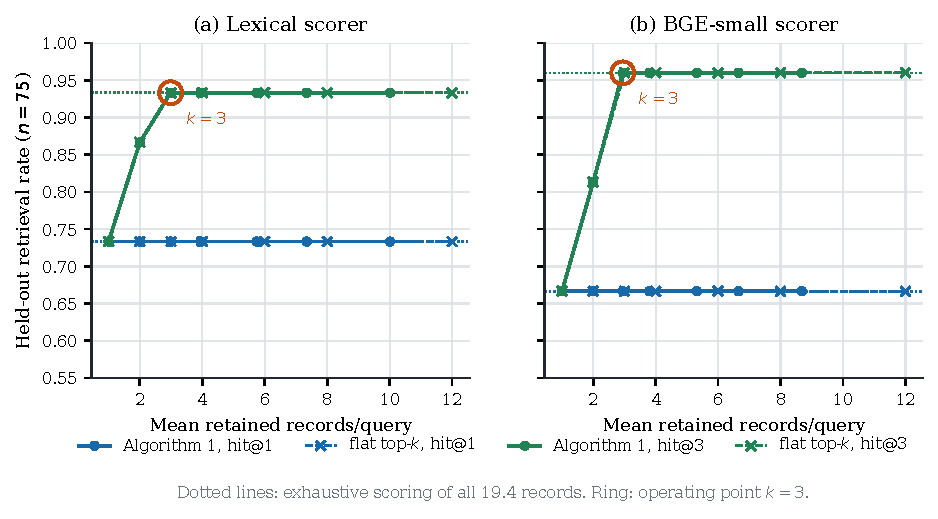
\includegraphics[width=0.90\textwidth]{figures/fig_scorer_frontiers.pdf}
\caption{Held-out quality versus retained records ($n=75$) as the budget $k$
varies. Algorithm~\ref{alg:query} (solid) and flat top-$k$ under the same scorer
(dashed) have identical hit@1 and hit@3 at every budget; dotted lines are
exhaustive scoring.}
\label{fig:frontier}
\end{figure*}

\subsection{Which components of the traversal matter}
\label{sec:ablation}
Figure~\ref{fig:mitigation} adds the components of Algorithm~\ref{alg:query} one
at a time to a fixed two-branch gate at $k=3$. On the development split, lexical
hit@3 rises from 0.700 to 0.740 with adaptive mass, to 0.840 with max-leaf branch
scores, and to 0.860 with the safety shortlist; BGE rises from 0.780 to 0.860,
almost entirely through the shortlist (for BGE the branch score is the
dev-selected summary score). On the held-out split the components act in the same way (lexical 0.787 to
0.933, BGE 0.813 to 0.960); there adaptive mass gives the largest lexical gain,
and for BGE the configured branch score adds nothing on either split. The confidence fallback did not
improve the development criterion and was disabled, so the selected configuration
never falls back; soft boundary membership was rejected for the same reason. The
components that matter are therefore the ones that make the traversal behave like
flat search: scoring branches by their best record and guaranteeing that the best
record survives.

\begin{figure*}[!tbp]
\centering
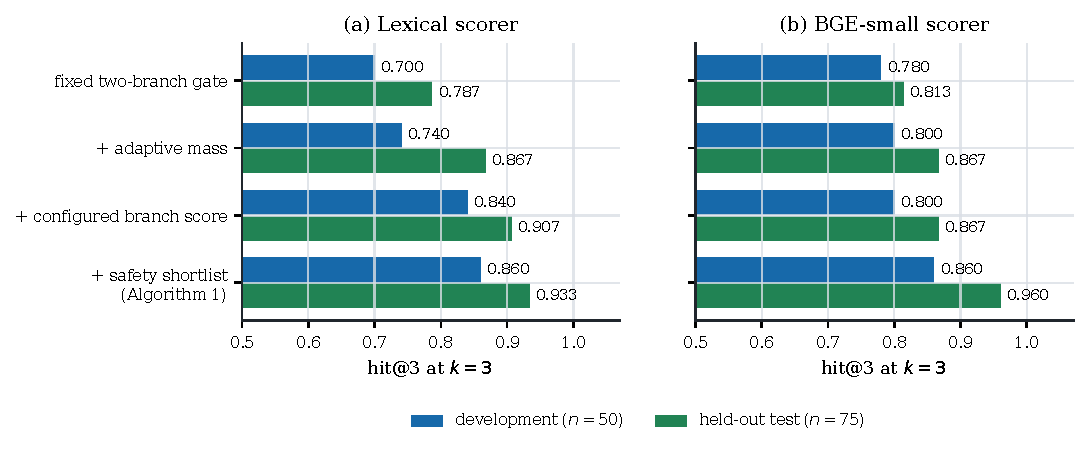
\includegraphics[width=0.84\textwidth]{figures/fig_mitigation_ablation.pdf}
\caption{Component ablation of Algorithm~\ref{alg:query} at $k=3$ on the
development split, where the configuration was chosen, and on the held-out split.
Each row adds one component to a fixed two-branch gate.}
\label{fig:mitigation}
\end{figure*}

The traversal parameters behave the same way (Fig.~\ref{fig:sensitivity}). On the
development split, hit@3 is unchanged across $\tau$, $T$, and the boundary width,
and drops only for a branch cap of one (0.84) or without the shortlist ($m=0$,
0.84). The budget $k$ is the only parameter that trades quality for records. With
$s\equiv r$ and $m\geq1$, a target ranked first by the scorer always survives, and
targets ranked second or third are lost only if they lie outside the kept
branches, so the gate parameters seldom matter.

\begin{figure*}[!tbp]
\centering
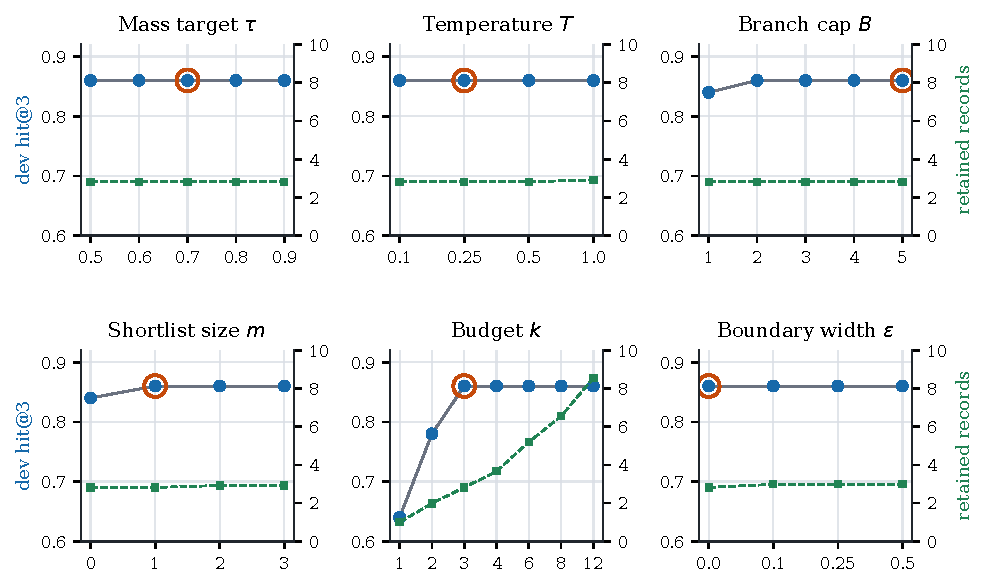
\includegraphics[width=0.88\textwidth]{figures/fig_sensitivity.pdf}
\caption{One-at-a-time sensitivity of development hit@3 (blue, left axis) and
retained records (green, right axis) to the traversal parameters (lexical scorer,
$n=50$). Rings mark the selected values.}
\label{fig:sensitivity}
\end{figure*}

All five held-out lexical misses (Table~\ref{tab:failures}) occur outdoors.
Because the traversal ranks every target exactly as flat top-3 does, all five are
failures of the scorer.
For two of them, restricting search to the zone that contains the target (an
oracle scope) recovers it, which shows that the correct zone would have removed a
distractor; the language-driven gate does not find that zone.

\begin{table}[!t]
\centering
\caption{All held-out lexical hit@3 misses ($n=75$). ``Oracle scope'' gives hit@3
when search is restricted to the zone that contains the target.}
\label{tab:failures}
\footnotesize
\begin{tabular}{lp{0.40\columnwidth}c}
\toprule
Scene & Query (abridged) & Oracle scope \\
\midrule
street & glass-block wall on the right & no \\
street & move between street levels & yes \\
street & utility access area & yes \\
street & street wayfinding marker & no \\
drone & rocky island surrounded by water & no \\
\bottomrule
\end{tabular}
\end{table}

\paragraph{Negative queries}
An abstention rule set on the development positives---abstain when the best proxy
score is at or below the fifth percentile of the development positives' best
scores---abstains on all 25 internal negatives with BGE, while answering 73 of the
75 held-out positives (hit@3 0.933 with abstentions counted as misses). The
lexical scorer abstains only when no token overlaps; it abstains on 22 of 25
negatives and answers every positive. Because the shortlist keeps the global best
record, flat search and the traversal make identical abstention decisions.

\subsection{The safety shortlist makes the hierarchy interchangeable}
\label{sec:hierarchies}
Table~\ref{tab:grid} compares the four hierarchies on all 125 positives under
three leaf scorers and two gates at $k=3$. Under Algorithm~\ref{alg:query}, no
hierarchy differs from the human zones in hit@1 or hit@3 under any scorer (every
paired interval contains zero), and none differs from flat search either: the
largest gaps, $-0.032$ for raw RGB-D under CLIP ($[-0.088,0.024]$) and $-0.024$
under BGE ($[-0.056,0.000]$), are within the resolution of the benchmark. The grid
uses max-leaf branch scores for every scorer and an untuned CLIP temperature of
0.01. Lexical
hit@3 is 0.904 for every hierarchy, equal to flat, and the values do not change at
$k=6$ or $k=12$. Under a weaker budget-filling gate, which orders branches by
max-leaf score but has no mass cut and no shortlist, point estimates spread
further---the human zones reach 0.864 under lexical and 0.552 under CLIP scoring,
and raw RGB-D 0.848 under BGE---while the coarse pose hierarchies stay close to
flat because they are nearly flat; at $k=3$ none of these differences is
significant at $n=125$.

\begin{table}[!t]
\centering
\caption{Hierarchy--scorer grid on 125 positives: hit@3 at $k=3$ under
Algorithm~\ref{alg:query} and under a budget-filling gate without mass cut or
shortlist. ``Br.'' is the number of top-level branches over the five
scenes.}
\label{tab:grid}
\footnotesize
\setlength{\tabcolsep}{2.2pt}
\begin{tabular}{lcccccccc}
\toprule
& & \multicolumn{3}{c}{Algorithm~\ref{alg:query}} & &
\multicolumn{3}{c}{Budget-filling gate} \\
\cmidrule{3-5}\cmidrule{7-9}
Hierarchy & Br. & Lex. & BGE & CLIP & & Lex. & BGE & CLIP \\
\midrule
Flat (no hierarchy) & -- & 0.904 & 0.928 & 0.624 & & 0.904 & 0.928 & 0.624 \\
Manual zones & 26 & 0.904 & 0.920 & 0.600 & & 0.864 & 0.880 & 0.552 \\
Pose only & 10 & 0.904 & 0.920 & 0.624 & & 0.888 & 0.880 & 0.624 \\
Pose+semantic & 8 & 0.904 & 0.920 & 0.624 & & 0.920 & 0.896 & 0.624 \\
Raw RGB-D & 27 & 0.904 & 0.904 & 0.592 & & 0.880 & 0.848 & 0.592 \\
\bottomrule
\end{tabular}
\end{table}

A fixed-width gate magnifies the dependence on the hierarchy. When only the two
best branches are kept and there is no shortlist (Fig.~\ref{fig:automatic}), the
target lies outside the kept branches for 21 of 125 queries with the human zones,
for 29 with raw RGB-D clusters, and for 2 with either pose hierarchy. CLIP hit@3
is 0.624 for flat search, 0.592 for the human zones, and 0.528 for raw clusters;
raw clusters are significantly worse than flat search ($-0.096$, 95\% CI
$[-0.168,-0.032]$) but not significantly worse than the human zones ($-0.064$,
$[-0.136,0.008]$). Replacing the fixed cut by Algorithm~\ref{alg:query} closes the
gap to flat search for every hierarchy within the resolution of the benchmark.

\begin{figure*}[!tbp]
\centering
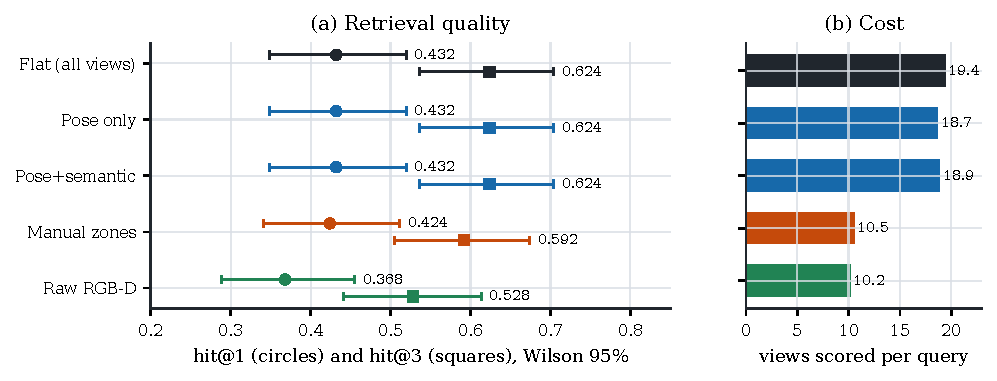
\includegraphics[width=0.84\textwidth]{figures/fig_raw_rgbd_hierarchy.pdf}
\caption{Fixed two-branch gate with the CLIP scorer (125 positives), an ablation
that Algorithm~\ref{alg:query} replaces. (a) hit@1 and hit@3 with Wilson 95\%
intervals; (b) views scored per query.}
\label{fig:automatic}
\end{figure*}

\paragraph{Construction cost and structure}
Pose-only construction for all five scenes takes 0.8\,ms, pose+semantic 6.3\,ms,
and raw RGB-D construction a median of 17\,s (12--23\,s over three runs on a shared
CPU; 97 images). The automatic
hierarchies agree with the human zones only moderately (Fig.~\ref{fig:structure}):
macro pairwise F1 is 0.588 for pose only, 0.570 for pose+semantic, and 0.487 for
raw RGB-D, against size-matched random partitions of 0.541, 0.563, and 0.366 and
a best attainable disjoint score of 0.877. The pose scores are close to random
because a single-branch scene scores the same as its random baseline.
Table~\ref{tab:constants} shows that the construction constants change structure
more than retrieval: under CLIP and the budget-filling gate, hit@3 stays within
0.568--0.632 over all tested values, while pairwise F1 ranges from 0.314 to
0.600.

\begin{figure}[!tbp]
\centering
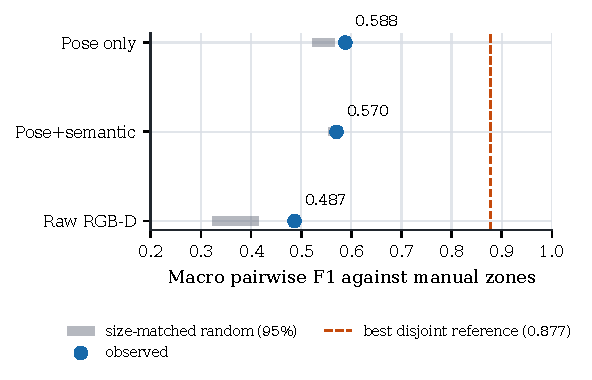
\includegraphics[width=0.98\columnwidth]{figures/fig_structure_controls.pdf}
\caption{Structural agreement (macro pairwise F1) of automatic hierarchies with
the human zones, beside cluster-size-matched random partitions and the best
disjoint projection of the overlapping human zones.}
\label{fig:structure}
\end{figure}

\begin{table*}[!t]
\centering
\caption{Construction constants (125 positives; CLIP scorer, budget-filling gate,
$k=3$). Defaults in bold. The minimum-cluster rule is not part of the released
constructor and was added for this sweep.}
\label{tab:constants}
\footnotesize
\begin{tabular}{lllll}
\toprule
Hierarchy & Constant & Values & F1 & hit@3 \\
\midrule
Pose only & $\alpha$ & 2, 2.5, 3, \textbf{3.5}, 4, 5 & 0.475--0.600 & 0.576--0.624 \\
Raw RGB-D & $K_{\max}$ & $n/4$, $\boldsymbol{n/3}$, $n/2$ & 0.496, 0.487, 0.314 & 0.608, 0.592, 0.568 \\
Raw RGB-D & min.\ views & \textbf{none}, 2, 3, 4 & 0.487--0.545 & 0.592--0.632 \\
Raw RGB-D & pose weight & 0, 0.25, \textbf{0.5}, 1 & 0.487--0.497 & 0.592 \\
Raw RGB-D & depth weight & 0, 0.1, \textbf{0.2}, 0.5 & 0.487--0.499 & 0.592--0.608 \\
\bottomrule
\end{tabular}
\end{table*}

\subsection{Scope, not similarity, limits retrieval at scale}
\label{sec:scale}
Figure~\ref{fig:scale} measures expression retrieval on pools of up to 155,535
records. At the largest pool, exact dense BGE retrieval obtains hit@3 0.236 and
HNSW~\cite{hnsw2020} 0.228; restricting search to the correct scene---an oracle
that assumes the scan ID is known---raises hit@3 to 0.948 while scoring 284
records. Of the flat misses at this pool, 96.9\% have all three returned
expressions in other scenes (96.6\% over all pools): the difficulty of this task is scope.

A language-only scene hierarchy does not recover that gain.
Algorithm~\ref{alg:query} over scene branches, tuned on disjoint queries, at best
matches flat search. With max-leaf branch scores it returns the flat result
(hit@3 0.234 in the same run as flat 0.234) but still scores every record. With
scene-summary scores and a three-record HNSW shortlist it obtains 0.232 (paired
difference $-0.002$, 95\% CI $[-0.012,0.008]$) while computing about 2,080 vector
similarities instead of 155,535. Without the shortlist its hit@3 falls to 0.116,
and at the largest pool its gate selects the query's own scene for only
3--27\% of queries, depending on the configuration. The retained accuracy therefore comes from the approximate shortlist, not from
the scene gate. HNSW alone obtains 0.228 in a separate run with about 584
distance computations. The summary configuration with a single branch and a
three-record shortlist was added to the tuning grid after inspecting tuning
results, but before any evaluation query was scored. Flat
hit@3 at the largest pool varies between 0.234 and 0.242 across runs because many
Sr3D+ template expressions tie exactly.

\begin{figure*}[!tbp]
\centering
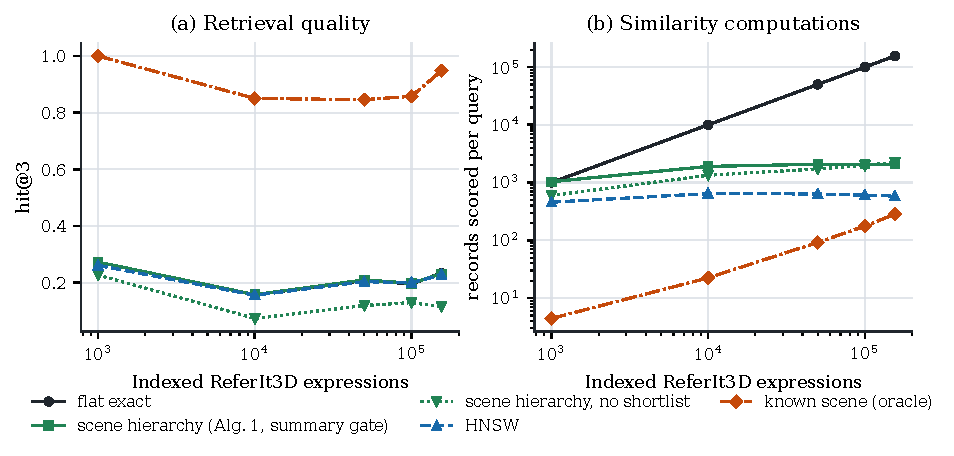
\includegraphics[width=0.96\textwidth]{figures/fig_public_scale_ann.pdf}
\caption{Expression retrieval over nested ReferIt3D pools (query expression
removed; a hit is another expression of the same scene and object). (a) hit@3;
(b) similarity computations per query (for HNSW: computed distances; for the
scene hierarchy: branch summaries, HNSW distances, and rescored records). The known-scene control assumes the scan ID
is known.}
\label{fig:scale}
\end{figure*}

\subsection{Object grounding}
\label{sec:objects}
Table~\ref{tab:objects} reports object grounding. On oracle ScanNet maps,
Algorithm~\ref{alg:query} with the object scorer reaches Recall@1 and Acc@0.25 of
0.604, matching flat lexical Acc@0.25 (0.604; flat Recall@1 0.625), while scoring
21.3 instead of 49.0 objects per query; Replica is a ceiling at 1.000 for every method in Table~\ref{tab:objects}. On predicted maps, accuracy is bounded by perception. On ScanNet, flat and
hierarchical BGE both place a box with IoU$\geq$0.25 for 6 of 48 queries, whereas
the same scorer reaches 17 of 48 (0.354) on the oracle map, and even the top three BGE candidates contain a box with IoU$\geq$0.25 for only
9 of 48 queries. With corrected ground
truth, native ConceptGraphs reaches Acc@0.25 of 0.271 on Replica (0.063 before the
correction). The paired BGE runs on Replica predicted maps could not be recomputed from the saved outputs and are omitted. On the 8 negatives per track,
lexical variants abstain because no token overlaps (negative accuracy 1.000);
embedding scorers and native ConceptGraphs never abstain (0.000).

\begin{table*}[!t]
\centering
\caption{Object grounding over positive queries. Objects: mean objects scored per
query. ScanNet queries were used during scorer development (in-sample). Predicted
maps are ConceptGraphs maps; Replica uses the corrected ground truth.
$^\ast$Spatial median-split hierarchy with $\tau=0.7$, $m=1$; it scores all cached
proxies and keeps 3 objects.}
\label{tab:objects}
\footnotesize
\begin{tabular}{lllcccc}
\toprule
Map & Dataset ($n$) & Method & R@1 & Acc@0.25 & Acc@0.5 & Objects \\
\midrule
oracle & ScanNet (48) & flat lexical + relations & 0.625 & 0.604 & -- & 49.0 \\
oracle & ScanNet (48) & Algorithm~\ref{alg:query} + relations & 0.604 & 0.604 & -- & 21.3 \\
oracle & ScanNet (48) & flat BGE & 0.333 & 0.354 & 0.333 & 49.0 \\
oracle & Replica (48) & all methods & 1.000 & 1.000 & 1.000 & 30.3--71.9 \\
\midrule
predicted & ScanNet (48) & flat BGE & -- & 0.125 & 0.021 & 50.4 \\
predicted & ScanNet (48) & hierarchical BGE$^\ast$ & -- & 0.125 & 0.021 & 50.4 \\
predicted & ScanNet (48) & native ConceptGraphs & -- & 0.063 & 0.000 & -- \\
predicted & Replica (48) & native ConceptGraphs & -- & 0.271 & 0.146 & -- \\
\bottomrule
\end{tabular}
\end{table*}

LangSplat~\cite{langsplat2024} was run once, on ScanNet 0011\_00 with six
queries, 3,000 instead of 30,000 optimization iterations, and a 6\,GB GPU; it
selected an expected view for 4 of 6 queries and outputs points rather than boxes.
We report it only as evidence that the pipeline runs on our data. We did not run
BBQ, whose released evaluation uses a different map and LLM protocol, so its
published numbers are not comparable with ours.

% =========================================================================
\section{Discussion}
\label{sec:discussion}
% =========================================================================

\subsection{What the results say about spatial language interfaces}
\paragraph{The reasoner should read little, and a flat cheap-first cascade
decides what well}
The clearest result is that the expensive model does not need the scene. With a
7B instruction model, a cached BGE ranking that passes about half of the records
halves tokens and latency at a hit@3 cost whose interval ends at 0.067, and a
three-record context raises the model's answer accuracy by 0.12. The limiting
factor is the recall of the cheap stage, which is 0.96 at three records on this
benchmark. Designers of spatial language interfaces can therefore spend their
effort on the first-stage ranking and on the budget rather than on the reasoner's
context window.

\paragraph{Spatial hierarchy is a representation, not a retrieval gain}
We found no setting in which the hierarchy selected better evidence than the flat
ranking of the same proxy at the same budget: not with lexical, dense,
image--text, or LLM scorers, not with human or automatic zones, and not at 155,535
records. The components that make the traversal competitive---max-leaf scoring
and the safety shortlist---are exactly those that make it reproduce the flat
ranking, and the one component that could add scope, the language-driven gate,
chose the correct scene for at most 27\% of queries at the largest pool. A hierarchy
should therefore be kept for what it provides independently of ranking: a
traceable route, an interface for spatial scoping by an external signal, and
structure for summaries. If a hierarchy is used for pruning, the shortlist is not
optional: without it, a gate loses up to a tenth of hit@3.

\paragraph{Scope is valuable when it comes from outside the query}
The scale study isolates a failure mode of flat retrieval that grows with the
collection: short descriptions are equally plausible in many scenes, and almost
every miss is an other-scene record. Knowing the scene lifts hit@3 from 0.236 to
0.948, whereas inferring it from the query text does not. Scope should therefore
come from localization, user context, or the robot's position, and the hierarchy
is the natural place to apply it.

\paragraph{Human zones are not needed for pruning} Under the proposed traversal, pose-only hierarchies built in under a millisecond
and raw RGB-D clusters were interchangeable with human-authored zones. Because the
shortlist removes the dependence on branch quality, manual zoning can be skipped.

\paragraph{Perception and evaluation dominate end-to-end grounding}
On predicted maps, every retrieval method was bounded by the map, and a single
unrotated box import had understated Replica accuracy about fourfold. Retrieval
methods for 3D grounding should report oracle- and predicted-map results with the
same scorer and verify their ground truth by passing it through the evaluator.

\subsection{Threats to validity} \emph{Internal validity.} Traversal parameters were selected on a development
split frozen before tuning, and all comparisons are paired, but the test split has
75 positives, so differences of a few points cannot be resolved. The internal
queries and labels were written by the authors, and the ScanNet object queries
were used while the object scorer was developed. \emph{Construct validity.}
Retained records and tokens measure what the reasoner reads, not monetary cost;
latencies were measured on one consumer GPU without a serving framework,
while other experiments shared the machine, so only their ratios are informative.
\emph{External validity.} The internal benchmark has five scenes rendered
from reconstructions, with renderer-derived depth, the scale study
uses expressions rather than boxes, the predicted-map results rest on one
perception system with sparse frames, and the largest reasoner has 7B parameters.
The conclusion that hierarchy does not beat a flat cascade holds for the scorers
and budgets tested; a proxy that encodes geometry the leaf scorer lacks could
behave differently.

% =========================================================================
\section{Reproducibility and Data Availability}
\label{sec:repro}
% =========================================================================
Code, the 150 queries with expected views and splits, the authored view
records and camera poses, per-query traces (branch probabilities, retained IDs,
token counts, latencies, and model scores), the corrected Replica ground-truth
import, and the scripts that regenerate every figure and table are released. The
rendered RGB-D views are not redistributed (see Ethics and Consent). The ReferIt3D, ScanNet, and Replica
data are available from their original providers under their licenses; we
release only derived records and identifiers. The models are
\path{Qwen/Qwen2.5-7B-Instruct} revision
\texttt{a09a35458c702b33eeac\allowbreak c393d103063234e8bc28} (bfloat16), the saved
\path{Qwen/Qwen2.5-1.5B-Instruct} revision
\texttt{989aa7980e4cf806f80c\allowbreak 7fef2b1adb7bc71aa306} runs,
\path{BAAI/bge-small-en-v1.5} (FastEmbed ONNX export), and
\path{openai/clip-vit-base-patch32}. The release is available at
\url{https://github.com/LeoVesinML/beyond-proximity-release}. LLM experiments ran on an Apple M4 Pro (14 CPU
cores, 48\,GB unified memory) using its GPU; the saved 1.5B runs used a CPU. Tokens
of non-LLM contexts are counted with \texttt{tiktoken} \texttt{cl100k\_base}.

\section*{Ethics and Consent}
The internal benchmark contains no images of people captured by the authors;
all views are renders of existing 3D Gaussian splatting reconstructions. We
inspected every released view: none shows an identifiable person, and the only
vehicle, in one street view, has no legible license plate. Some views show
framed photographs and exhibition panels that are part of the reconstructed
interiors. The reconstructions were published by their authors on the SuperSplat
platform, whose terms of use allow others to use, reproduce, and create derivative
works from publicly posted content with attribution to its authors; we credit
each scene's author in the release. We do not redistribute the reconstructions
or the rendered views; the released records, poses, and results contain no image
content.

% =========================================================================
\section{Conclusion}
% =========================================================================
We asked how much of a 3D scene a language model must read and whether a spatial
hierarchy chooses that evidence better than a flat cascade. Under same-scorer,
matched-budget controls, the answer to the first question is ``very little'': a
cheap proxy that passes half of the records preserves most of the reasoner's
recall while halving its cost, and a three-record context improves its answers. The
answer to the second is ``no'': the recall-controlled traversal ranks every target as the flat ranking of
its proxy does, its safety shortlist makes the hierarchy
interchangeable, and a language-driven scene gate does not recover the large scope
gain that external localization provides at 155,535 records. Hierarchies remain
useful as an interface for externally supplied scope and for traceable routes,
and pose-based hierarchies provide them without annotation.

\section*{Acknowledgment}
OpenAI Codex~\cite{openai2025codex} assisted with drafting and language editing of
an earlier version of the manuscript and with experiment and figure-export code.
The authors reviewed all generated text and code.

\appendices
\section{Place vocabulary of the raw RGB-D constructor}
\label{app:vocab}
Clusters are named with the CLIP prompt ``a photograph of a \{label\}'' and the
following 20 labels: auditorium, banquet hall, conference room, corridor,
entrance, exhibition gallery, facade, garden, information desk, lobby, lounge,
museum display, outdoor plaza, reception desk, service counter, stage, street,
theater seating, walkway, and wayfinding area. Five of them (facade, garden,
outdoor plaza, street, walkway) describe outdoor places.

\bibliographystyle{IEEEtran}
\bibliography{refs}

\EOD

\end{document}
